\documentclass[parskip]{scrartcl}
\usepackage[margin=15mm]{geometry}
\usepackage{tikz}
\usepackage{pifont}

\begin{document}
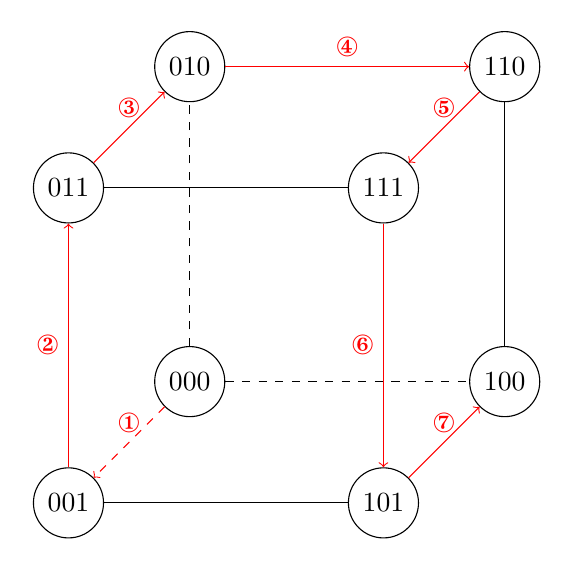
\begin{tikzpicture}
\tikzstyle{conjecture}=[draw,circle,solid]
\node[conjecture] (000) at (0, 0, 0) {000};
\node[conjecture] (001) at (0, 0, 4) {001};
\node[conjecture] (011) at (0, 4, 4) {011};
\node[conjecture] (010) at (0, 4, 0) {010};
\node[conjecture] (110) at (4, 4, 0) {110};
\node[conjecture] (111) at (4, 4, 4) {111};
\node[conjecture] (101) at (4, 0, 4) {101};
\node[conjecture] (100) at (4, 0, 0) {100};

\draw[dashed] (000) -- (100);
\draw[dashed] (000) -- (010);
\draw (011) -- (111);
\draw (101) -- (001);
\draw (110) -- (100);


\draw[dashed, red, ->] (000) -- node[above] {\ding{172}} (001);
\draw[red, ->] (001) -- node[left]  {\ding{173}} (011);
\draw[red, ->] (011) -- node[above] {\ding{174}} (010);
\draw[red, ->] (010) -- node[above] {\ding{175}} (110);
\draw[red, ->] (110) -- node[above] {\ding{176}} (111);
\draw[red, ->] (111) -- node[left]  {\ding{177}} (101);
\draw[red, ->] (101) -- node[above] {\ding{178}} (100);

\end{tikzpicture}

\end{document}
